\documentclass[12pt,a4paper,oneside,ngerman]{article} 
\usepackage[left=3cm,right=3cm,top=2.5cm]{geometry} % Groesse der Seitenraender definieren
\usepackage[utf8]{inputenc} % utf8 encoding
\usepackage{hyperref}
\usepackage{ngerman}
\usepackage{graphicx}
\usepackage{underscore}
\usepackage{tikz} % Automaten, Graphen, ... zeichnen
\usepackage{tikz-qtree} % Paket fuer Tikz Graphen-Baeume
\usetikzlibrary{arrows,shapes,automata} % Bestimmte tikz-Befehle benutzen
\usepackage{amsmath,amssymb} % Mathe-Formeln und -Ausdruecke
\usepackage{listings} % Code-Ausschnitte einbinden
\usepackage{xcolor} % Eigene Farben definieren
\usepackage{colortbl} % Farben verwenden in Tabellen
\usepackage{wrapfig} % Bilder von Text umfliessen lassen
\usepackage{multicol} % Mehrspaltigen Text schreiben
\usepackage{stmaryrd} % Fuer Symbole wie zu Beispiel Widerspruchspfeil
\usepackage{caption}
\usepackage{totpages}

% Beliebige RGB Farben definieren:
\definecolor{gold}{rgb}{0.83, 0.69, 0.15}
\definecolor{magenta}{rgb}{0.79, 0.08, 0.48}

% Titel in Kopfzeilen
\usepackage{fancyhdr}
\pagestyle{fancy}
\fancyhf{}
\setlength{\headheight}{20pt}

% Seitenumbrueche werden nicht mehr eingerueckt
\setlength{\parindent}{0em}


% % % % % % % % % % % % % % % % % % % % % % % % % % % % % % 
%Variablen
% % % % % % % % % % % % % % % % % % % % % % % % % % % % % % 
\newcommand{\fach}{Objektorientierte Modellierung und Programmierung}
\newcommand{\dokumentenTitel}{Abgabe Uebungsblatt Nr.01}
\newcommand{\Abgabe}{28.04.2020, 12:00 Uhr}
\newcommand{\memberOne}{Marius Birk}
\newcommand{\memberTwo}{Pieter Vogt}


\newcommand{\tutor}{ Florian Brandt }
% % % % % % % % % % % % % % % % % % % % % % % % % % % % % 

% Kopfzeile auf jeder Seite:
\fancyhead[R]{\dokumentenTitel} % Dokument-Titel
\fancyhead[C]{}
\fancyhead[L]{\memberOne, \memberTwo} % Autorennamen
\renewcommand{\headrulewidth}{0.4pt} %obere Trennlinie

% Fußzeile auf jeder Seite:
\fancyfoot[C]{Seite \thepage \ von \ref{TotPages}} %Seitennummer
\renewcommand{\footrulewidth}{0.4pt} %untere Trennlinie

% Nun beginnt das eigentliche Dokument
\begin{document}
	\thispagestyle{plain} % Keine Kopfzeile auf erster Seite, aber Seitenzahl wird angezeigt
	
	\begin{multicols}{2} % Beginnt zweispaltigen Text fuer Header auf erster Seite
		\hspace{-1cm} % Linken Header-Teil 1cm nach links schieben.
		% Tabelle fuer linke Seite vom Header der ersten Seite
		\begin{tabular}{ll} % Mit l werden die Eintraege linksbuendig
			Autoren: & \memberOne \\ % Zwischen jeder Spalte ein & einfuegen
			& \memberTwo \\
			% beendet eine Tabellenzeile 
			Tutor: & \tutor \\  
		\end{tabular}
		
		\columnbreak % Nun beginnt die rechte Seite des Headers
		\hspace{-1cm} % Rechten Header-Teil 1cm nach links schieben.
		% Tabelle fuer rechte Seite vom Header der ersten Seite
		\begin{tabular}{ll} % p{1cm} bewirkt, dass die rechte Spalte 6cm breit ist.
			Abgabe: & \Abgabe \\ % Zwischen jeder Spalte ein & einfuege
			Punkte: &  
			%Mit diesem Befehl wird die Zeilenhoehe der folgenden Tabelle um 20% erhoeht.   
			\renewcommand{\arraystretch}{1.2} 
			% Nun kommt eine innere Tabelle in der aeusseren Tabelle, mit der eine Punktetabelle fuer den Tutor erstellt wird:  
			\begin{tabular}{|p{0.8cm}|p{0.8cm}|p{0.8cm}|p{0.8cm}|p{0.8cm}|p{0.8cm}|}
				\hline a & b & c & d & e & $\sum\limits^{ }$ \\ \hline
				& & & & & \\ \hline    
			\end{tabular} \\
		\end{tabular}
		
	\end{multicols} % Beendet zweispaltigen Text
	
	\begin{center}
		\Large{\fach} \\
		\LARGE{\dokumentenTitel} \\
		\small
		$($Alle allgemeinen Definitionen aus der Vorlesung haben in diesem Dokument bestand, es sei den sie erhalten eine explizit andere Definition.$)$
    \end{center}

	\section{Aufgabe 1}
		\subsection{Teilaufgabe a} 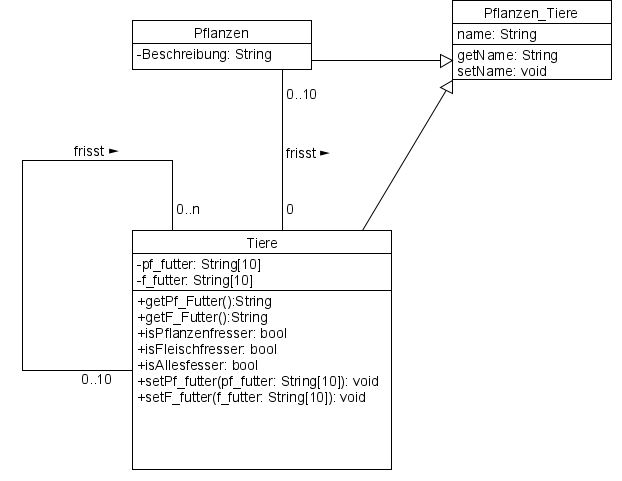
\includegraphics{ohnefohnepf}
		\subsection{Teilaufgabe b}  Siehe beigefügte Datei Pflanzen_Tiere.java.\\
		\subsection{Teilaufgabe c}  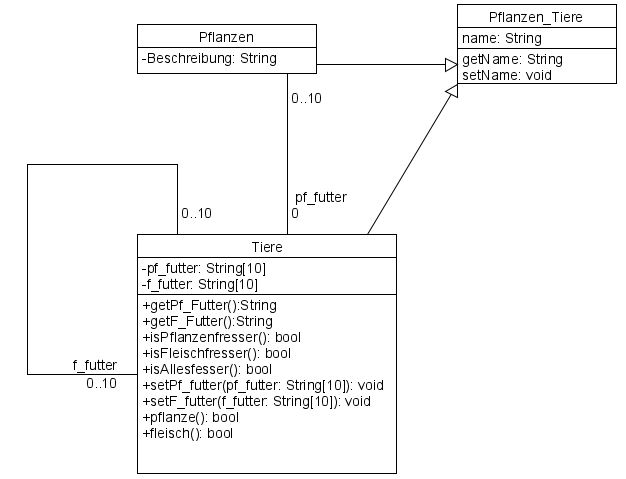
\includegraphics{UML Diagramm}
		\subsection{Teilaufgabe d}  Siehe beigefügte Datei Bio_Test.java.\\
		\subsection{Teilaufgabe e}  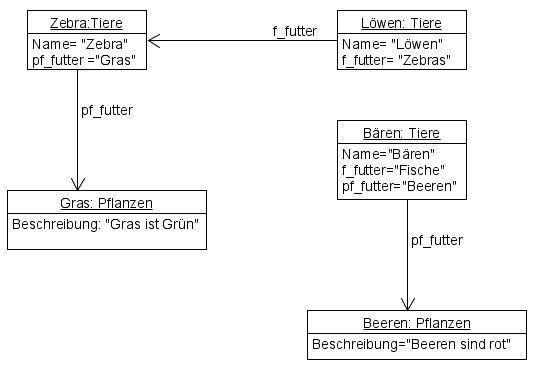
\includegraphics{objektdiagramm}


	
\end{document}
